\documentclass[1p]{elsarticle_modified}
%\bibliographystyle{elsarticle-num}

%\usepackage[colorlinks]{hyperref}
%\usepackage{abbrmath_seonhwa} %\Abb, \Ascr, \Acal ,\Abf, \Afrak
\usepackage{amsfonts}
\usepackage{amssymb}
\usepackage{amsmath}
\usepackage{amsthm}
\usepackage{scalefnt}
\usepackage{amsbsy}
\usepackage{kotex}
\usepackage{caption}
\usepackage{subfig}
\usepackage{color}
\usepackage{graphicx}
\usepackage{xcolor} %% white, black, red, green, blue, cyan, magenta, yellow
\usepackage{float}
\usepackage{setspace}
\usepackage{hyperref}

\usepackage{tikz}
\usetikzlibrary{arrows}

\usepackage{multirow}
\usepackage{array} % fixed length table
\usepackage{hhline}

%%%%%%%%%%%%%%%%%%%%%
\makeatletter
\renewcommand*\env@matrix[1][\arraystretch]{%
	\edef\arraystretch{#1}%
	\hskip -\arraycolsep
	\let\@ifnextchar\new@ifnextchar
	\array{*\c@MaxMatrixCols c}}
\makeatother %https://tex.stackexchange.com/questions/14071/how-can-i-increase-the-line-spacing-in-a-matrix
%%%%%%%%%%%%%%%

\usepackage[normalem]{ulem}

\newcommand{\msout}[1]{\ifmmode\text{\sout{\ensuremath{#1}}}\else\sout{#1}\fi}
%SOURCE: \msout is \stkout macro in https://tex.stackexchange.com/questions/20609/strikeout-in-math-mode

\newcommand{\cancel}[1]{
	\ifmmode
	{\color{red}\msout{#1}}
	\else
	{\color{red}\sout{#1}}
	\fi
}

\newcommand{\add}[1]{
	{\color{blue}\uwave{#1}}
}

\newcommand{\replace}[2]{
	\ifmmode
	{\color{red}\msout{#1}}{\color{blue}\uwave{#2}}
	\else
	{\color{red}\sout{#1}}{\color{blue}\uwave{#2}}
	\fi
}

\newcommand{\Sol}{\mathcal{S}} %segment
\newcommand{\D}{D} %diagram
\newcommand{\A}{\mathcal{A}} %arc


%%%%%%%%%%%%%%%%%%%%%%%%%%%%%5 test

\def\sl{\operatorname{\textup{SL}}(2,\Cbb)}
\def\psl{\operatorname{\textup{PSL}}(2,\Cbb)}
\def\quan{\mkern 1mu \triangleright \mkern 1mu}

\theoremstyle{definition}
\newtheorem{thm}{Theorem}[section]
\newtheorem{prop}[thm]{Proposition}
\newtheorem{lem}[thm]{Lemma}
\newtheorem{ques}[thm]{Question}
\newtheorem{cor}[thm]{Corollary}
\newtheorem{defn}[thm]{Definition}
\newtheorem{exam}[thm]{Example}
\newtheorem{rmk}[thm]{Remark}
\newtheorem{alg}[thm]{Algorithm}

\newcommand{\I}{\sqrt{-1}}
\begin{document}

%\begin{frontmatter}
%
%\title{Boundary parabolic representations of knots up to 8 crossings}
%
%%% Group authors per affiliation:
%\author{Yunhi Cho} 
%\address{Department of Mathematics, University of Seoul, Seoul, Korea}
%\ead{yhcho@uos.ac.kr}
%
%
%\author{Seonhwa Kim} %\fnref{s_kim}}
%\address{Center for Geometry and Physics, Institute for Basic Science, Pohang, 37673, Korea}
%\ead{ryeona17@ibs.re.kr}
%
%\author{Hyuk Kim}
%\address{Department of Mathematical Sciences, Seoul National University, Seoul 08826, Korea}
%\ead{hyukkim@snu.ac.kr}
%
%\author{Seokbeom Yoon}
%\address{Department of Mathematical Sciences, Seoul National University, Seoul, 08826,  Korea}
%\ead{sbyoon15@snu.ac.kr}
%
%\begin{abstract}
%We find all boundary parabolic representation of knots up to 8 crossings.
%
%\end{abstract}
%\begin{keyword}
%    \MSC[2010] 57M25 
%\end{keyword}
%
%\end{frontmatter}

%\linenumbers
%\tableofcontents
%
\newcommand\colored[1]{\textcolor{white}{\rule[-0.35ex]{0.8em}{1.4ex}}\kern-0.8em\color{red} #1}%
%\newcommand\colored[1]{\textcolor{white}{ #1}\kern-2.17ex	\textcolor{white}{ #1}\kern-1.81ex	\textcolor{white}{ #1}\kern-2.15ex\color{red}#1	}

{\Large $\underline{12n_{0584}~(K12n_{0584})}$}

\setlength{\tabcolsep}{10pt}
\renewcommand{\arraystretch}{1.6}
\vspace{1cm}\begin{tabular}{m{100pt}>{\centering\arraybackslash}m{274pt}}
\multirow{5}{120pt}{
	\centering
	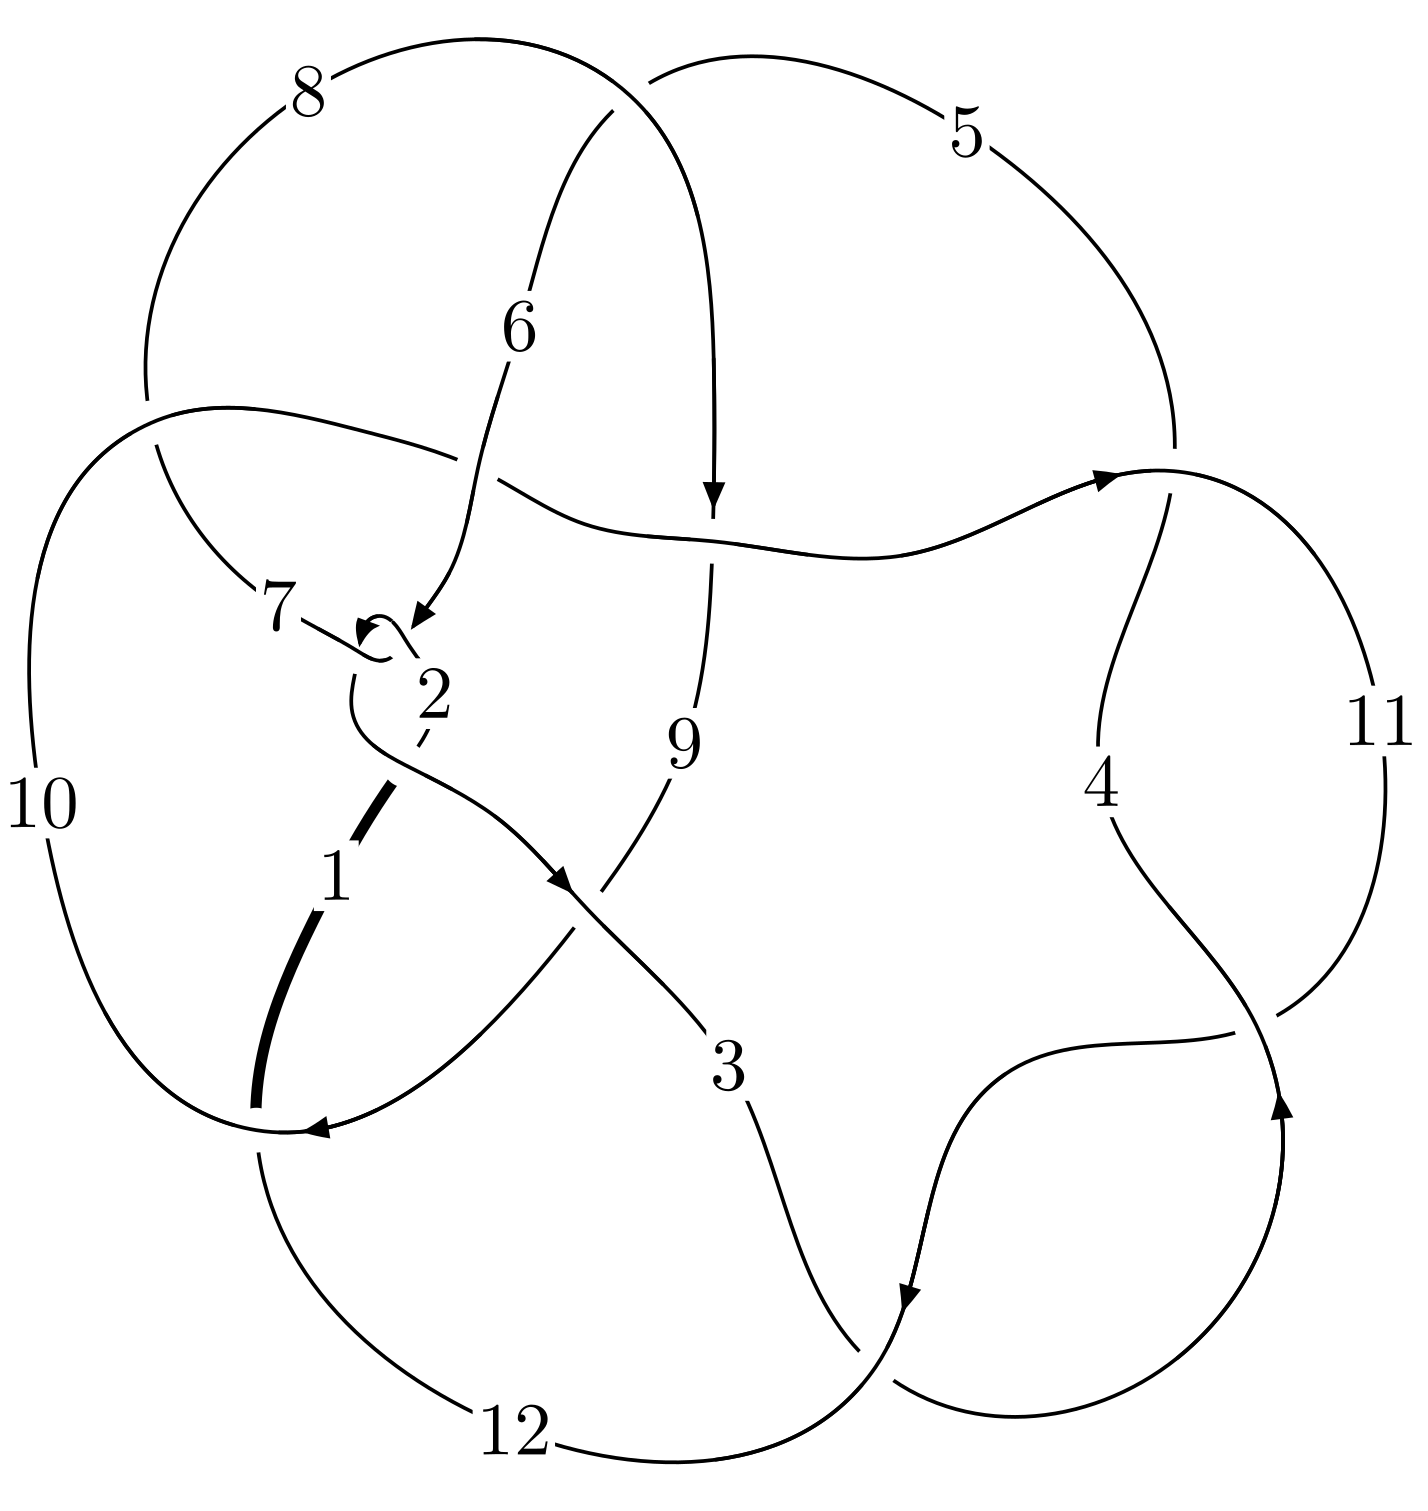
\includegraphics[width=112pt]{../../../GIT/diagram.site/Diagrams/png/2673_12n_0584.png}\\
\ \ \ A knot diagram\footnotemark}&
\allowdisplaybreaks
\textbf{Linearized knot diagam} \\
\cline{2-2}
 &
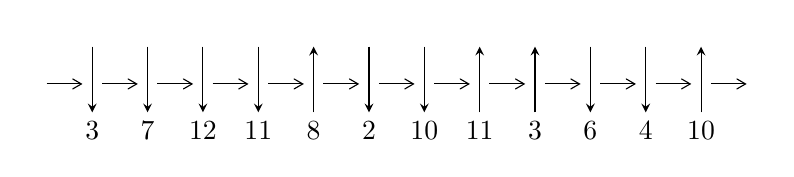
\begin{tikzpicture}[x=20pt, y=17pt]
	% nodes
	\node (C0) at (0, 0) {};
	\node (C1) at (1, 0) {};
	\node (C1U) at (1, +1) {};
	\node (C1D) at (1, -1) {3};

	\node (C2) at (2, 0) {};
	\node (C2U) at (2, +1) {};
	\node (C2D) at (2, -1) {7};

	\node (C3) at (3, 0) {};
	\node (C3U) at (3, +1) {};
	\node (C3D) at (3, -1) {12};

	\node (C4) at (4, 0) {};
	\node (C4U) at (4, +1) {};
	\node (C4D) at (4, -1) {11};

	\node (C5) at (5, 0) {};
	\node (C5U) at (5, +1) {};
	\node (C5D) at (5, -1) {8};

	\node (C6) at (6, 0) {};
	\node (C6U) at (6, +1) {};
	\node (C6D) at (6, -1) {2};

	\node (C7) at (7, 0) {};
	\node (C7U) at (7, +1) {};
	\node (C7D) at (7, -1) {10};

	\node (C8) at (8, 0) {};
	\node (C8U) at (8, +1) {};
	\node (C8D) at (8, -1) {11};

	\node (C9) at (9, 0) {};
	\node (C9U) at (9, +1) {};
	\node (C9D) at (9, -1) {3};

	\node (C10) at (10, 0) {};
	\node (C10U) at (10, +1) {};
	\node (C10D) at (10, -1) {6};

	\node (C11) at (11, 0) {};
	\node (C11U) at (11, +1) {};
	\node (C11D) at (11, -1) {4};

	\node (C12) at (12, 0) {};
	\node (C12U) at (12, +1) {};
	\node (C12D) at (12, -1) {10};
	\node (C13) at (13, 0) {};

	% arrows
	\draw[->,>={angle 60}]
	(C0) edge (C1) (C1) edge (C2) (C2) edge (C3) (C3) edge (C4) (C4) edge (C5) (C5) edge (C6) (C6) edge (C7) (C7) edge (C8) (C8) edge (C9) (C9) edge (C10) (C10) edge (C11) (C11) edge (C12) (C12) edge (C13) ;	\draw[->,>=stealth]
	(C1U) edge (C1D) (C2U) edge (C2D) (C3U) edge (C3D) (C4U) edge (C4D) (C5D) edge (C5U) (C6U) edge (C6D) (C7U) edge (C7D) (C8D) edge (C8U) (C9D) edge (C9U) (C10U) edge (C10D) (C11U) edge (C11D) (C12D) edge (C12U) ;
	\end{tikzpicture} \\
\hhline{~~} \\& 
\textbf{Solving Sequence} \\ \cline{2-2} 
 &
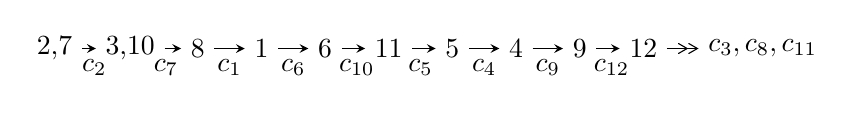
\begin{tikzpicture}[x=23pt, y=7pt]
	% node
	\node (A0) at (-1/8, 0) {2,7};
	\node (A1) at (17/16, 0) {3,10};
	\node (A2) at (17/8, 0) {8};
	\node (A3) at (25/8, 0) {1};
	\node (A4) at (33/8, 0) {6};
	\node (A5) at (41/8, 0) {11};
	\node (A6) at (49/8, 0) {5};
	\node (A7) at (57/8, 0) {4};
	\node (A8) at (65/8, 0) {9};
	\node (A9) at (73/8, 0) {12};
	\node (C1) at (1/2, -1) {$c_{2}$};
	\node (C2) at (13/8, -1) {$c_{7}$};
	\node (C3) at (21/8, -1) {$c_{1}$};
	\node (C4) at (29/8, -1) {$c_{6}$};
	\node (C5) at (37/8, -1) {$c_{10}$};
	\node (C6) at (45/8, -1) {$c_{5}$};
	\node (C7) at (53/8, -1) {$c_{4}$};
	\node (C8) at (61/8, -1) {$c_{9}$};
	\node (C9) at (69/8, -1) {$c_{12}$};
	\node (A10) at (11, 0) {$c_{3},c_{8},c_{11}$};

	% edge
	\draw[->,>=stealth]	
	(A0) edge (A1) (A1) edge (A2) (A2) edge (A3) (A3) edge (A4) (A4) edge (A5) (A5) edge (A6) (A6) edge (A7) (A7) edge (A8) (A8) edge (A9) ;
	\draw[->>,>={angle 60}]	
	(A9) edge (A10);
\end{tikzpicture} \\ 

\end{tabular} \\

\footnotetext{
The image of knot diagram is generated by the software ``\textbf{Draw programme}" developed by Andrew Bartholomew(\url{http://www.layer8.co.uk/maths/draw/index.htm\#Running-draw}), where we modified some parts for our purpose(\url{https://github.com/CATsTAILs/LinksPainter}).
}\phantom \\ \newline 
\centering \textbf{Ideals for irreducible components\footnotemark of $X_{\text{par}}$} 
 
\begin{align*}
I^u_{1}&=\langle 
-2.84207\times10^{81} u^{60}-2.95633\times10^{81} u^{59}+\cdots+5.11199\times10^{81} b-2.88400\times10^{82},\\
\phantom{I^u_{1}}&\phantom{= \langle  }-1.14386\times10^{81} u^{60}-4.62548\times10^{81} u^{59}+\cdots+1.06887\times10^{82} a-7.85278\times10^{82},\\
\phantom{I^u_{1}}&\phantom{= \langle  }u^{61}+u^{60}+\cdots-22 u-23\rangle \\
I^u_{2}&=\langle 
-17 u^{15}-11 u^{14}+\cdots+5 b+24,\;-38 u^{15}-24 u^{14}+\cdots+5 a+51,\\
\phantom{I^u_{2}}&\phantom{= \langle  }u^{16}-4 u^{14}- u^{13}+10 u^{12}+4 u^{11}-18 u^{10}-8 u^9+25 u^8+9 u^7-23 u^6-6 u^5+14 u^4+3 u^3-5 u^2- u+1\rangle \\
\\
\end{align*}
\raggedright * 2 irreducible components of $\dim_{\mathbb{C}}=0$, with total 77 representations.\\
\footnotetext{All coefficients of polynomials are rational numbers. But the coefficients are sometimes approximated in decimal forms when there is not enough margin.}
\newpage
\renewcommand{\arraystretch}{1}
\centering \section*{I. $I^u_{1}= \langle -2.84\times10^{81} u^{60}-2.96\times10^{81} u^{59}+\cdots+5.11\times10^{81} b-2.88\times10^{82},\;-1.14\times10^{81} u^{60}-4.63\times10^{81} u^{59}+\cdots+1.07\times10^{82} a-7.85\times10^{82},\;u^{61}+u^{60}+\cdots-22 u-23 \rangle$}
\flushleft \textbf{(i) Arc colorings}\\
\begin{tabular}{m{7pt} m{180pt} m{7pt} m{180pt} }
\flushright $a_{2}=$&$\begin{pmatrix}1\\0\end{pmatrix}$ \\
\flushright $a_{7}=$&$\begin{pmatrix}0\\u\end{pmatrix}$ \\
\flushright $a_{3}=$&$\begin{pmatrix}1\\u^2\end{pmatrix}$ \\
\flushright $a_{10}=$&$\begin{pmatrix}0.107015 u^{60}+0.432744 u^{59}+\cdots+11.5924 u+7.34680\\0.555961 u^{60}+0.578313 u^{59}+\cdots+13.5777 u+5.64164\end{pmatrix}$ \\
\flushright $a_{8}=$&$\begin{pmatrix}-1.63482 u^{60}-0.434066 u^{59}+\cdots-3.95439 u+24.4321\\-1.20730 u^{60}-0.120843 u^{59}+\cdots+1.65510 u+29.0484\end{pmatrix}$ \\
\flushright $a_{1}=$&$\begin{pmatrix}- u^2+1\\- u^4\end{pmatrix}$ \\
\flushright $a_{6}=$&$\begin{pmatrix}u\\u\end{pmatrix}$ \\
\flushright $a_{11}=$&$\begin{pmatrix}-0.525349 u^{60}+0.268729 u^{59}+\cdots+7.94097 u+14.3245\\-0.0764035 u^{60}+0.414298 u^{59}+\cdots+9.92621 u+12.6193\end{pmatrix}$ \\
\flushright $a_{5}=$&$\begin{pmatrix}0.132466 u^{60}-0.942714 u^{59}+\cdots-27.4934 u-9.73617\\0.157167 u^{60}-0.596294 u^{59}+\cdots-18.0455 u-3.48263\end{pmatrix}$ \\
\flushright $a_{4}=$&$\begin{pmatrix}-1.08158 u^{60}-0.482855 u^{59}+\cdots-14.9772 u+30.5122\\0.233874 u^{60}-0.223864 u^{59}+\cdots-8.46851 u-1.44589\end{pmatrix}$ \\
\flushright $a_{9}=$&$\begin{pmatrix}-0.504826 u^{60}+0.228474 u^{59}+\cdots+7.64215 u+9.19693\\-0.303905 u^{60}+0.301421 u^{59}+\cdots+8.47187 u+15.0158\end{pmatrix}$ \\
\flushright $a_{12}=$&$\begin{pmatrix}-1.28481 u^{60}+0.424922 u^{59}+\cdots+11.1040 u+38.8528\\-0.877631 u^{60}-0.0161271 u^{59}+\cdots+0.455782 u+24.0747\end{pmatrix}$\\&\end{tabular}
\flushleft \textbf{(ii) Obstruction class $= -1$}\\~\\
\flushleft \textbf{(iii) Cusp Shapes $= -0.265475 u^{60}+0.396204 u^{59}+\cdots+11.1890 u-16.1033$}\\~\\
\newpage\renewcommand{\arraystretch}{1}
\flushleft \textbf{(iv) u-Polynomials at the component}\newline \\
\begin{tabular}{m{50pt}|m{274pt}}
Crossings & \hspace{64pt}u-Polynomials at each crossing \\
\hline $$\begin{aligned}c_{1}\end{aligned}$$&$\begin{aligned}
&u^{61}+37 u^{60}+\cdots+3014 u+529
\end{aligned}$\\
\hline $$\begin{aligned}c_{2},c_{6}\end{aligned}$$&$\begin{aligned}
&u^{61}- u^{60}+\cdots-22 u+23
\end{aligned}$\\
\hline $$\begin{aligned}c_{3},c_{4},c_{11}\end{aligned}$$&$\begin{aligned}
&u^{61}-3 u^{60}+\cdots- u+1
\end{aligned}$\\
\hline $$\begin{aligned}c_{5}\end{aligned}$$&$\begin{aligned}
&u^{61}+5 u^{60}+\cdots+128 u+56
\end{aligned}$\\
\hline $$\begin{aligned}c_{7}\end{aligned}$$&$\begin{aligned}
&u^{61}+u^{60}+\cdots+4795 u-1559
\end{aligned}$\\
\hline $$\begin{aligned}c_{8}\end{aligned}$$&$\begin{aligned}
&u^{61}+3 u^{60}+\cdots+1189 u-103
\end{aligned}$\\
\hline $$\begin{aligned}c_{9}\end{aligned}$$&$\begin{aligned}
&u^{61}- u^{60}+\cdots-4288 u+1856
\end{aligned}$\\
\hline $$\begin{aligned}c_{10}\end{aligned}$$&$\begin{aligned}
&u^{61}+u^{60}+\cdots-19 u+1
\end{aligned}$\\
\hline $$\begin{aligned}c_{12}\end{aligned}$$&$\begin{aligned}
&u^{61}- u^{60}+\cdots-120835 u+26113
\end{aligned}$\\
\hline
\end{tabular}\\~\\
\newpage\renewcommand{\arraystretch}{1}
\flushleft \textbf{(v) Riley Polynomials at the component}\newline \\
\begin{tabular}{m{50pt}|m{274pt}}
Crossings & \hspace{64pt}Riley Polynomials at each crossing \\
\hline $$\begin{aligned}c_{1}\end{aligned}$$&$\begin{aligned}
&y^{61}-17 y^{60}+\cdots+10572802 y-279841
\end{aligned}$\\
\hline $$\begin{aligned}c_{2},c_{6}\end{aligned}$$&$\begin{aligned}
&y^{61}-37 y^{60}+\cdots+3014 y-529
\end{aligned}$\\
\hline $$\begin{aligned}c_{3},c_{4},c_{11}\end{aligned}$$&$\begin{aligned}
&y^{61}+45 y^{60}+\cdots-61 y-1
\end{aligned}$\\
\hline $$\begin{aligned}c_{5}\end{aligned}$$&$\begin{aligned}
&y^{61}+47 y^{60}+\cdots-214112 y-3136
\end{aligned}$\\
\hline $$\begin{aligned}c_{7}\end{aligned}$$&$\begin{aligned}
&y^{61}-31 y^{60}+\cdots+107411875 y-2430481
\end{aligned}$\\
\hline $$\begin{aligned}c_{8}\end{aligned}$$&$\begin{aligned}
&y^{61}+49 y^{60}+\cdots+350761 y-10609
\end{aligned}$\\
\hline $$\begin{aligned}c_{9}\end{aligned}$$&$\begin{aligned}
&y^{61}+51 y^{60}+\cdots-57040896 y-3444736
\end{aligned}$\\
\hline $$\begin{aligned}c_{10}\end{aligned}$$&$\begin{aligned}
&y^{61}+15 y^{60}+\cdots+51 y-1
\end{aligned}$\\
\hline $$\begin{aligned}c_{12}\end{aligned}$$&$\begin{aligned}
&y^{61}+55 y^{60}+\cdots+971678005 y-681888769
\end{aligned}$\\
\hline
\end{tabular}\\~\\
\newpage\flushleft \textbf{(vi) Complex Volumes and Cusp Shapes}
$$\begin{array}{c|c|c}  
\text{Solutions to }I^u_{1}& \I (\text{vol} + \sqrt{-1}CS) & \text{Cusp shape}\\
 \hline 
\begin{aligned}
u &= -0.959151 + 0.188873 I \\
a &= \phantom{-}0.71607 - 2.11317 I \\
b &= \phantom{-}0.427222 - 1.250120 I\end{aligned}
 & -0.40672 + 5.49798 I & -3.46413 - 7.66192 I \\ \hline\begin{aligned}
u &= -0.959151 - 0.188873 I \\
a &= \phantom{-}0.71607 + 2.11317 I \\
b &= \phantom{-}0.427222 + 1.250120 I\end{aligned}
 & -0.40672 - 5.49798 I & -3.46413 + 7.66192 I \\ \hline\begin{aligned}
u &= -0.934743 + 0.424563 I \\
a &= -0.220618 + 0.026435 I \\
b &= -1.043970 + 0.429854 I\end{aligned}
 & \phantom{-}1.60124 + 2.09731 I & -0.52172 - 3.57800 I \\ \hline\begin{aligned}
u &= -0.934743 - 0.424563 I \\
a &= -0.220618 - 0.026435 I \\
b &= -1.043970 - 0.429854 I\end{aligned}
 & \phantom{-}1.60124 - 2.09731 I & -0.52172 + 3.57800 I \\ \hline\begin{aligned}
u &= -0.205719 + 0.937770 I \\
a &= \phantom{-}0.007890 - 1.331690 I \\
b &= -0.780566 - 0.133806 I\end{aligned}
 & -2.24217 + 2.51722 I & -4.13220 - 2.03658 I \\ \hline\begin{aligned}
u &= -0.205719 - 0.937770 I \\
a &= \phantom{-}0.007890 + 1.331690 I \\
b &= -0.780566 + 0.133806 I\end{aligned}
 & -2.24217 - 2.51722 I & -4.13220 + 2.03658 I \\ \hline\begin{aligned}
u &= \phantom{-}0.162902 + 1.031490 I \\
a &= -0.260817 - 1.260900 I \\
b &= \phantom{-}0.544283 - 0.172289 I\end{aligned}
 & -6.40462 + 3.64805 I & -6.12698 - 2.44450 I \\ \hline\begin{aligned}
u &= \phantom{-}0.162902 - 1.031490 I \\
a &= -0.260817 + 1.260900 I \\
b &= \phantom{-}0.544283 + 0.172289 I\end{aligned}
 & -6.40462 - 3.64805 I & -6.12698 + 2.44450 I \\ \hline\begin{aligned}
u &= \phantom{-}0.941999 + 0.077674 I \\
a &= -1.08751 - 1.37046 I \\
b &= -1.055650 - 0.247755 I\end{aligned}
 & -1.84937 - 1.06710 I & -7.68501 + 0.20822 I \\ \hline\begin{aligned}
u &= \phantom{-}0.941999 - 0.077674 I \\
a &= -1.08751 + 1.37046 I \\
b &= -1.055650 + 0.247755 I\end{aligned}
 & -1.84937 + 1.06710 I & -7.68501 - 0.20822 I\\
 \hline 
 \end{array}$$\newpage$$\begin{array}{c|c|c}  
\text{Solutions to }I^u_{1}& \I (\text{vol} + \sqrt{-1}CS) & \text{Cusp shape}\\
 \hline 
\begin{aligned}
u &= -0.937483 + 0.102090 I \\
a &= \phantom{-}0.484123 + 0.573834 I \\
b &= \phantom{-}0.98031 - 1.45346 I\end{aligned}
 & \phantom{-}4.81378 + 0.51083 I & -5.07863 + 3.86372 I \\ \hline\begin{aligned}
u &= -0.937483 - 0.102090 I \\
a &= \phantom{-}0.484123 - 0.573834 I \\
b &= \phantom{-}0.98031 + 1.45346 I\end{aligned}
 & \phantom{-}4.81378 - 0.51083 I & -5.07863 - 3.86372 I \\ \hline\begin{aligned}
u &= \phantom{-}1.008430 + 0.362616 I \\
a &= -1.000510 - 0.605838 I \\
b &= -2.33129 - 0.84687 I\end{aligned}
 & \phantom{-}0.01276 - 7.14753 I & -2.20400 + 9.04049 I \\ \hline\begin{aligned}
u &= \phantom{-}1.008430 - 0.362616 I \\
a &= -1.000510 + 0.605838 I \\
b &= -2.33129 + 0.84687 I\end{aligned}
 & \phantom{-}0.01276 + 7.14753 I & -2.20400 - 9.04049 I \\ \hline\begin{aligned}
u &= \phantom{-}0.643141 + 0.668518 I \\
a &= -0.716958 + 0.049390 I \\
b &= \phantom{-}0.318873 + 0.601995 I\end{aligned}
 & \phantom{-}1.75152 - 2.53902 I & \phantom{-}1.27559 + 4.14078 I \\ \hline\begin{aligned}
u &= \phantom{-}0.643141 - 0.668518 I \\
a &= -0.716958 - 0.049390 I \\
b &= \phantom{-}0.318873 - 0.601995 I\end{aligned}
 & \phantom{-}1.75152 + 2.53902 I & \phantom{-}1.27559 - 4.14078 I \\ \hline\begin{aligned}
u &= \phantom{-}0.753203 + 0.517931 I \\
a &= -0.102774 + 0.952076 I \\
b &= -0.367431 + 1.094570 I\end{aligned}
 & -1.66195 - 1.20234 I & -8.53362 + 3.15271 I \\ \hline\begin{aligned}
u &= \phantom{-}0.753203 - 0.517931 I \\
a &= -0.102774 - 0.952076 I \\
b &= -0.367431 - 1.094570 I\end{aligned}
 & -1.66195 + 1.20234 I & -8.53362 - 3.15271 I \\ \hline\begin{aligned}
u &= \phantom{-}0.910915\phantom{ +0.000000I} \\
a &= \phantom{-}0.473770\phantom{ +0.000000I} \\
b &= \phantom{-}1.07394\phantom{ +0.000000I}\end{aligned}
 & -1.32772\phantom{ +0.000000I} & -8.18480\phantom{ +0.000000I} \\ \hline\begin{aligned}
u &= -0.153240 + 1.083330 I \\
a &= \phantom{-}0.430101 - 1.162100 I \\
b &= -0.365491 - 0.155347 I\end{aligned}
 & -2.13464 - 9.66628 I & -2.68073 + 5.89377 I\\
 \hline 
 \end{array}$$\newpage$$\begin{array}{c|c|c}  
\text{Solutions to }I^u_{1}& \I (\text{vol} + \sqrt{-1}CS) & \text{Cusp shape}\\
 \hline 
\begin{aligned}
u &= -0.153240 - 1.083330 I \\
a &= \phantom{-}0.430101 + 1.162100 I \\
b &= -0.365491 + 0.155347 I\end{aligned}
 & -2.13464 + 9.66628 I & -2.68073 - 5.89377 I \\ \hline\begin{aligned}
u &= \phantom{-}1.115530 + 0.094811 I \\
a &= -1.368590 + 0.050906 I \\
b &= -2.09969 - 0.80379 I\end{aligned}
 & -3.09183 - 0.94578 I & -8.08189 - 0.53980 I \\ \hline\begin{aligned}
u &= \phantom{-}1.115530 - 0.094811 I \\
a &= -1.368590 - 0.050906 I \\
b &= -2.09969 + 0.80379 I\end{aligned}
 & -3.09183 + 0.94578 I & -8.08189 + 0.53980 I \\ \hline\begin{aligned}
u &= -0.768294 + 0.427994 I \\
a &= -0.233622 - 0.672878 I \\
b &= -0.887371 + 0.068293 I\end{aligned}
 & \phantom{-}1.25803 + 1.85767 I & \phantom{-}3.29586 - 4.00259 I \\ \hline\begin{aligned}
u &= -0.768294 - 0.427994 I \\
a &= -0.233622 + 0.672878 I \\
b &= -0.887371 - 0.068293 I\end{aligned}
 & \phantom{-}1.25803 - 1.85767 I & \phantom{-}3.29586 + 4.00259 I \\ \hline\begin{aligned}
u &= -0.223321 + 0.842928 I \\
a &= \phantom{-}0.897998 + 0.077975 I \\
b &= \phantom{-}0.036178 + 0.399582 I\end{aligned}
 & \phantom{-}3.62908 + 2.32516 I & \phantom{-}4.48467 - 2.65480 I \\ \hline\begin{aligned}
u &= -0.223321 - 0.842928 I \\
a &= \phantom{-}0.897998 - 0.077975 I \\
b &= \phantom{-}0.036178 - 0.399582 I\end{aligned}
 & \phantom{-}3.62908 - 2.32516 I & \phantom{-}4.48467 + 2.65480 I \\ \hline\begin{aligned}
u &= \phantom{-}0.889016 + 0.747517 I \\
a &= \phantom{-}0.607385 - 0.821852 I \\
b &= \phantom{-}1.395130 + 0.149616 I\end{aligned}
 & \phantom{-}9.07136 - 2.85087 I & \phantom{-}9.78334 + 0. I\phantom{ +0.000000I} \\ \hline\begin{aligned}
u &= \phantom{-}0.889016 - 0.747517 I \\
a &= \phantom{-}0.607385 + 0.821852 I \\
b &= \phantom{-}1.395130 - 0.149616 I\end{aligned}
 & \phantom{-}9.07136 + 2.85087 I & \phantom{-}9.78334 + 0. I\phantom{ +0.000000I} \\ \hline\begin{aligned}
u &= \phantom{-}1.130530 + 0.481440 I \\
a &= -1.302640 + 0.202022 I \\
b &= -1.82636 + 0.28273 I\end{aligned}
 & -3.38137 - 2.36705 I & \phantom{-0.000000 } 0\\
 \hline 
 \end{array}$$\newpage$$\begin{array}{c|c|c}  
\text{Solutions to }I^u_{1}& \I (\text{vol} + \sqrt{-1}CS) & \text{Cusp shape}\\
 \hline 
\begin{aligned}
u &= \phantom{-}1.130530 - 0.481440 I \\
a &= -1.302640 - 0.202022 I \\
b &= -1.82636 - 0.28273 I\end{aligned}
 & -3.38137 + 2.36705 I & \phantom{-0.000000 } 0 \\ \hline\begin{aligned}
u &= -1.164240 + 0.451221 I \\
a &= \phantom{-}1.44291 - 0.32158 I \\
b &= \phantom{-}2.22996 - 0.29926 I\end{aligned}
 & -3.53482 + 5.70296 I & \phantom{-0.000000 } 0 \\ \hline\begin{aligned}
u &= -1.164240 - 0.451221 I \\
a &= \phantom{-}1.44291 + 0.32158 I \\
b &= \phantom{-}2.22996 + 0.29926 I\end{aligned}
 & -3.53482 - 5.70296 I & \phantom{-0.000000 } 0 \\ \hline\begin{aligned}
u &= -0.686059 + 0.293330 I \\
a &= -1.01986 + 1.45708 I \\
b &= -0.74714 + 1.69501 I\end{aligned}
 & \phantom{-}0.27896 - 3.26826 I & -2.74807 - 0.82015 I \\ \hline\begin{aligned}
u &= -0.686059 - 0.293330 I \\
a &= -1.01986 - 1.45708 I \\
b &= -0.74714 - 1.69501 I\end{aligned}
 & \phantom{-}0.27896 + 3.26826 I & -2.74807 + 0.82015 I \\ \hline\begin{aligned}
u &= -1.228430 + 0.253328 I \\
a &= \phantom{-}1.293940 - 0.408857 I \\
b &= \phantom{-}2.05763 - 0.91740 I\end{aligned}
 & -3.69197 + 4.91295 I & \phantom{-0.000000 } 0 \\ \hline\begin{aligned}
u &= -1.228430 - 0.253328 I \\
a &= \phantom{-}1.293940 + 0.408857 I \\
b &= \phantom{-}2.05763 + 0.91740 I\end{aligned}
 & -3.69197 - 4.91295 I & \phantom{-0.000000 } 0 \\ \hline\begin{aligned}
u &= -1.225300 + 0.340151 I \\
a &= \phantom{-}1.215390 - 0.430859 I \\
b &= \phantom{-}1.97241 - 0.78995 I\end{aligned}
 & -3.61600 + 4.89193 I & \phantom{-0.000000 } 0 \\ \hline\begin{aligned}
u &= -1.225300 - 0.340151 I \\
a &= \phantom{-}1.215390 + 0.430859 I \\
b &= \phantom{-}1.97241 + 0.78995 I\end{aligned}
 & -3.61600 - 4.89193 I & \phantom{-0.000000 } 0 \\ \hline\begin{aligned}
u &= \phantom{-}1.306570 + 0.385321 I \\
a &= \phantom{-}0.772428 + 0.105070 I \\
b &= \phantom{-}1.58309 - 0.82825 I\end{aligned}
 & -6.95611 - 6.96468 I & \phantom{-0.000000 } 0\\
 \hline 
 \end{array}$$\newpage$$\begin{array}{c|c|c}  
\text{Solutions to }I^u_{1}& \I (\text{vol} + \sqrt{-1}CS) & \text{Cusp shape}\\
 \hline 
\begin{aligned}
u &= \phantom{-}1.306570 - 0.385321 I \\
a &= \phantom{-}0.772428 - 0.105070 I \\
b &= \phantom{-}1.58309 + 0.82825 I\end{aligned}
 & -6.95611 + 6.96468 I & \phantom{-0.000000 } 0 \\ \hline\begin{aligned}
u &= -0.060803 + 0.628747 I \\
a &= -0.53802 + 1.47756 I \\
b &= -0.127042 + 0.473478 I\end{aligned}
 & -0.44119 - 1.56470 I & -4.17028 + 3.88456 I \\ \hline\begin{aligned}
u &= -0.060803 - 0.628747 I \\
a &= -0.53802 - 1.47756 I \\
b &= -0.127042 - 0.473478 I\end{aligned}
 & -0.44119 + 1.56470 I & -4.17028 - 3.88456 I \\ \hline\begin{aligned}
u &= -0.922764 + 1.032820 I \\
a &= \phantom{-}0.199690 + 0.204735 I \\
b &= \phantom{-}0.403670 + 0.238476 I\end{aligned}
 & \phantom{-}4.00754 + 3.70557 I & \phantom{-0.000000 } 0 \\ \hline\begin{aligned}
u &= -0.922764 - 1.032820 I \\
a &= \phantom{-}0.199690 - 0.204735 I \\
b &= \phantom{-}0.403670 - 0.238476 I\end{aligned}
 & \phantom{-}4.00754 - 3.70557 I & \phantom{-0.000000 } 0 \\ \hline\begin{aligned}
u &= \phantom{-}0.457781 + 0.408457 I \\
a &= \phantom{-}0.56646 + 2.03842 I \\
b &= \phantom{-}0.511340 - 0.004138 I\end{aligned}
 & \phantom{-}1.59167 + 3.79186 I & \phantom{-}1.89741 - 1.93857 I \\ \hline\begin{aligned}
u &= \phantom{-}0.457781 - 0.408457 I \\
a &= \phantom{-}0.56646 - 2.03842 I \\
b &= \phantom{-}0.511340 + 0.004138 I\end{aligned}
 & \phantom{-}1.59167 - 3.79186 I & \phantom{-}1.89741 + 1.93857 I \\ \hline\begin{aligned}
u &= -1.262930 + 0.592649 I \\
a &= -1.262610 - 0.329157 I \\
b &= -2.25061 + 0.25489 I\end{aligned}
 & -5.42549 + 3.10789 I & \phantom{-0.000000 } 0 \\ \hline\begin{aligned}
u &= -1.262930 - 0.592649 I \\
a &= -1.262610 + 0.329157 I \\
b &= -2.25061 - 0.25489 I\end{aligned}
 & -5.42549 - 3.10789 I & \phantom{-0.000000 } 0 \\ \hline\begin{aligned}
u &= -1.36643 + 0.38967 I \\
a &= -0.765288 - 0.003995 I \\
b &= -1.47807 - 0.79705 I\end{aligned}
 & -11.38250 + 1.28053 I & \phantom{-0.000000 } 0\\
 \hline 
 \end{array}$$\newpage$$\begin{array}{c|c|c}  
\text{Solutions to }I^u_{1}& \I (\text{vol} + \sqrt{-1}CS) & \text{Cusp shape}\\
 \hline 
\begin{aligned}
u &= -1.36643 - 0.38967 I \\
a &= -0.765288 + 0.003995 I \\
b &= -1.47807 + 0.79705 I\end{aligned}
 & -11.38250 - 1.28053 I & \phantom{-0.000000 } 0 \\ \hline\begin{aligned}
u &= \phantom{-}1.29707 + 0.58314 I \\
a &= \phantom{-}1.350370 - 0.078787 I \\
b &= \phantom{-}2.35665 + 0.43807 I\end{aligned}
 & -9.91993 - 9.45681 I & \phantom{-0.000000 } 0 \\ \hline\begin{aligned}
u &= \phantom{-}1.29707 - 0.58314 I \\
a &= \phantom{-}1.350370 + 0.078787 I \\
b &= \phantom{-}2.35665 - 0.43807 I\end{aligned}
 & -9.91993 + 9.45681 I & \phantom{-0.000000 } 0 \\ \hline\begin{aligned}
u &= -1.31022 + 0.58889 I \\
a &= -1.322870 + 0.107133 I \\
b &= -2.34658 + 0.59048 I\end{aligned}
 & -5.7532 + 15.6192 I & \phantom{-0.000000 } 0 \\ \hline\begin{aligned}
u &= -1.31022 - 0.58889 I \\
a &= -1.322870 - 0.107133 I \\
b &= -2.34658 - 0.59048 I\end{aligned}
 & -5.7532 - 15.6192 I & \phantom{-0.000000 } 0 \\ \hline\begin{aligned}
u &= \phantom{-}1.37880 + 0.46708 I \\
a &= -0.888680 - 0.525147 I \\
b &= -1.34840 - 0.85335 I\end{aligned}
 & -1.29850 - 7.17717 I & \phantom{-0.000000 } 0 \\ \hline\begin{aligned}
u &= \phantom{-}1.37880 - 0.46708 I \\
a &= -0.888680 + 0.525147 I \\
b &= -1.34840 + 0.85335 I\end{aligned}
 & -1.29850 + 7.17717 I & \phantom{-0.000000 } 0 \\ \hline\begin{aligned}
u &= \phantom{-}1.42356 + 0.37284 I \\
a &= \phantom{-}0.707166 - 0.088229 I \\
b &= \phantom{-}1.34948 - 0.74233 I\end{aligned}
 & -7.38726 + 4.45354 I & \phantom{-0.000000 } 0 \\ \hline\begin{aligned}
u &= \phantom{-}1.42356 - 0.37284 I \\
a &= \phantom{-}0.707166 + 0.088229 I \\
b &= \phantom{-}1.34948 + 0.74233 I\end{aligned}
 & -7.38726 - 4.45354 I & \phantom{-0.000000 } 0 \\ \hline\begin{aligned}
u &= -0.054872 + 0.484805 I \\
a &= -1.31570 + 1.52600 I \\
b &= -0.147524 + 0.297815 I\end{aligned}
 & -0.23274 - 1.52753 I & -1.85083 + 4.54656 I\\
 \hline 
 \end{array}$$\newpage$$\begin{array}{c|c|c}  
\text{Solutions to }I^u_{1}& \I (\text{vol} + \sqrt{-1}CS) & \text{Cusp shape}\\
 \hline 
\begin{aligned}
u &= -0.054872 - 0.484805 I \\
a &= -1.31570 - 1.52600 I \\
b &= -0.147524 - 0.297815 I\end{aligned}
 & -0.23274 + 1.52753 I & -1.85083 - 4.54656 I\\
 \hline 
 \end{array}$$\newpage\newpage\renewcommand{\arraystretch}{1}
\centering \section*{II. $I^u_{2}= \langle -17 u^{15}-11 u^{14}+\cdots+5 b+24,\;-38 u^{15}-24 u^{14}+\cdots+5 a+51,\;u^{16}-4 u^{14}+\cdots- u+1 \rangle$}
\flushleft \textbf{(i) Arc colorings}\\
\begin{tabular}{m{7pt} m{180pt} m{7pt} m{180pt} }
\flushright $a_{2}=$&$\begin{pmatrix}1\\0\end{pmatrix}$ \\
\flushright $a_{7}=$&$\begin{pmatrix}0\\u\end{pmatrix}$ \\
\flushright $a_{3}=$&$\begin{pmatrix}1\\u^2\end{pmatrix}$ \\
\flushright $a_{10}=$&$\begin{pmatrix}\frac{38}{5} u^{15}+\frac{24}{5} u^{14}+\cdots-\frac{41}{5} u-\frac{51}{5}\\\frac{17}{5} u^{15}+\frac{11}{5} u^{14}+\cdots-\frac{14}{5} u-\frac{24}{5}\end{pmatrix}$ \\
\flushright $a_{8}=$&$\begin{pmatrix}3 u^{15}+2 u^{14}+\cdots+2 u+1\\-\frac{6}{5} u^{15}-\frac{3}{5} u^{14}+\cdots+\frac{17}{5} u+\frac{27}{5}\end{pmatrix}$ \\
\flushright $a_{1}=$&$\begin{pmatrix}- u^2+1\\- u^4\end{pmatrix}$ \\
\flushright $a_{6}=$&$\begin{pmatrix}u\\u\end{pmatrix}$ \\
\flushright $a_{11}=$&$\begin{pmatrix}\frac{42}{5} u^{15}+\frac{31}{5} u^{14}+\cdots-\frac{49}{5} u-\frac{64}{5}\\\frac{21}{5} u^{15}+\frac{18}{5} u^{14}+\cdots-\frac{22}{5} u-\frac{37}{5}\end{pmatrix}$ \\
\flushright $a_{5}=$&$\begin{pmatrix}-11.6000 u^{15}-7.80000 u^{14}+\cdots+11.2000 u+15.2000\\-5.80000 u^{15}-4.40000 u^{14}+\cdots+4.60000 u+7.60000\end{pmatrix}$ \\
\flushright $a_{4}=$&$\begin{pmatrix}-6.20000 u^{15}-4.60000 u^{14}+\cdots+6.40000 u+11.4000\\-5.20000 u^{15}-2.60000 u^{14}+\cdots+5.40000 u+6.40000\end{pmatrix}$ \\
\flushright $a_{9}=$&$\begin{pmatrix}\frac{33}{5} u^{15}+\frac{24}{5} u^{14}+\cdots-\frac{41}{5} u-\frac{51}{5}\\\frac{12}{5} u^{15}+\frac{11}{5} u^{14}+\cdots-\frac{9}{5} u-\frac{24}{5}\end{pmatrix}$ \\
\flushright $a_{12}=$&$\begin{pmatrix}\frac{14}{5} u^{15}+\frac{2}{5} u^{14}+\cdots-\frac{33}{5} u-\frac{18}{5}\\\frac{14}{5} u^{15}+\frac{7}{5} u^{14}+\cdots-\frac{28}{5} u-\frac{23}{5}\end{pmatrix}$\\&\end{tabular}
\flushleft \textbf{(ii) Obstruction class $= 1$}\\~\\
\flushleft \textbf{(iii) Cusp Shapes $= -\frac{96}{5} u^{15}-\frac{53}{5} u^{14}+68 u^{13}+\frac{301}{5} u^{12}-\frac{752}{5} u^{11}-166 u^{10}+\frac{1158}{5} u^9+\frac{1467}{5} u^8-\frac{1404}{5} u^7-\frac{1716}{5} u^6+204 u^5+\frac{1261}{5} u^4-\frac{501}{5} u^3-\frac{611}{5} u^2+\frac{57}{5} u+\frac{132}{5}$}\\~\\
\newpage\renewcommand{\arraystretch}{1}
\flushleft \textbf{(iv) u-Polynomials at the component}\newline \\
\begin{tabular}{m{50pt}|m{274pt}}
Crossings & \hspace{64pt}u-Polynomials at each crossing \\
\hline $$\begin{aligned}c_{1}\end{aligned}$$&$\begin{aligned}
&u^{16}-8 u^{15}+\cdots-11 u+1
\end{aligned}$\\
\hline $$\begin{aligned}c_{2}\end{aligned}$$&$\begin{aligned}
&u^{16}-4 u^{14}+\cdots- u+1
\end{aligned}$\\
\hline $$\begin{aligned}c_{3},c_{4}\end{aligned}$$&$\begin{aligned}
&u^{16}+2 u^{15}+\cdots+8 u+1
\end{aligned}$\\
\hline $$\begin{aligned}c_{5}\end{aligned}$$&$\begin{aligned}
&u^{16}+6 u^{14}+\cdots+8 u^2+1
\end{aligned}$\\
\hline $$\begin{aligned}c_{6}\end{aligned}$$&$\begin{aligned}
&u^{16}-4 u^{14}+\cdots+u+1
\end{aligned}$\\
\hline $$\begin{aligned}c_{7}\end{aligned}$$&$\begin{aligned}
&u^{16}-12 u^{15}+\cdots-8 u+1
\end{aligned}$\\
\hline $$\begin{aligned}c_{8}\end{aligned}$$&$\begin{aligned}
&u^{16}+4 u^{15}+\cdots-3 u^2+1
\end{aligned}$\\
\hline $$\begin{aligned}c_{9}\end{aligned}$$&$\begin{aligned}
&u^{16}+6 u^{14}+\cdots+u+1
\end{aligned}$\\
\hline $$\begin{aligned}c_{10}\end{aligned}$$&$\begin{aligned}
&u^{16}+8 u^{14}+\cdots+6 u^2+1
\end{aligned}$\\
\hline $$\begin{aligned}c_{11}\end{aligned}$$&$\begin{aligned}
&u^{16}-2 u^{15}+\cdots-8 u+1
\end{aligned}$\\
\hline $$\begin{aligned}c_{12}\end{aligned}$$&$\begin{aligned}
&u^{16}+2 u^{14}+\cdots+2 u+1
\end{aligned}$\\
\hline
\end{tabular}\\~\\
\newpage\renewcommand{\arraystretch}{1}
\flushleft \textbf{(v) Riley Polynomials at the component}\newline \\
\begin{tabular}{m{50pt}|m{274pt}}
Crossings & \hspace{64pt}Riley Polynomials at each crossing \\
\hline $$\begin{aligned}c_{1}\end{aligned}$$&$\begin{aligned}
&y^{16}+8 y^{15}+\cdots-3 y+1
\end{aligned}$\\
\hline $$\begin{aligned}c_{2},c_{6}\end{aligned}$$&$\begin{aligned}
&y^{16}-8 y^{15}+\cdots-11 y+1
\end{aligned}$\\
\hline $$\begin{aligned}c_{3},c_{4},c_{11}\end{aligned}$$&$\begin{aligned}
&y^{16}+18 y^{15}+\cdots-16 y+1
\end{aligned}$\\
\hline $$\begin{aligned}c_{5}\end{aligned}$$&$\begin{aligned}
&y^{16}+12 y^{15}+\cdots+16 y+1
\end{aligned}$\\
\hline $$\begin{aligned}c_{7}\end{aligned}$$&$\begin{aligned}
&y^{16}-2 y^{15}+\cdots+24 y+1
\end{aligned}$\\
\hline $$\begin{aligned}c_{8}\end{aligned}$$&$\begin{aligned}
&y^{16}+6 y^{15}+\cdots-6 y+1
\end{aligned}$\\
\hline $$\begin{aligned}c_{9}\end{aligned}$$&$\begin{aligned}
&y^{16}+12 y^{15}+\cdots+13 y+1
\end{aligned}$\\
\hline $$\begin{aligned}c_{10}\end{aligned}$$&$\begin{aligned}
&y^{16}+16 y^{15}+\cdots+12 y+1
\end{aligned}$\\
\hline $$\begin{aligned}c_{12}\end{aligned}$$&$\begin{aligned}
&y^{16}+4 y^{15}+\cdots-10 y+1
\end{aligned}$\\
\hline
\end{tabular}\\~\\
\newpage\flushleft \textbf{(vi) Complex Volumes and Cusp Shapes}
$$\begin{array}{c|c|c}  
\text{Solutions to }I^u_{2}& \I (\text{vol} + \sqrt{-1}CS) & \text{Cusp shape}\\
 \hline 
\begin{aligned}
u &= -0.913832 + 0.235082 I \\
a &= \phantom{-}0.128344 - 0.430133 I \\
b &= -0.51462 + 1.51604 I\end{aligned}
 & \phantom{-}5.04845 + 1.02692 I & \phantom{-}1.87205 - 8.56014 I \\ \hline\begin{aligned}
u &= -0.913832 - 0.235082 I \\
a &= \phantom{-}0.128344 + 0.430133 I \\
b &= -0.51462 - 1.51604 I\end{aligned}
 & \phantom{-}5.04845 - 1.02692 I & \phantom{-}1.87205 + 8.56014 I \\ \hline\begin{aligned}
u &= \phantom{-}0.781665 + 0.507913 I \\
a &= -0.442004 - 0.379613 I \\
b &= \phantom{-}0.243014 + 0.419895 I\end{aligned}
 & \phantom{-}0.13293 - 2.08915 I & -4.96987 + 3.94005 I \\ \hline\begin{aligned}
u &= \phantom{-}0.781665 - 0.507913 I \\
a &= -0.442004 + 0.379613 I \\
b &= \phantom{-}0.243014 - 0.419895 I\end{aligned}
 & \phantom{-}0.13293 + 2.08915 I & -4.96987 - 3.94005 I \\ \hline\begin{aligned}
u &= \phantom{-}0.902595 + 0.772917 I \\
a &= -0.745532 + 0.878575 I \\
b &= -1.53315 - 0.12089 I\end{aligned}
 & \phantom{-}8.66558 - 2.92614 I & -9.74877 + 4.50724 I \\ \hline\begin{aligned}
u &= \phantom{-}0.902595 - 0.772917 I \\
a &= -0.745532 - 0.878575 I \\
b &= -1.53315 + 0.12089 I\end{aligned}
 & \phantom{-}8.66558 + 2.92614 I & -9.74877 - 4.50724 I \\ \hline\begin{aligned}
u &= -1.141260 + 0.432326 I \\
a &= \phantom{-}1.52602 - 0.04764 I \\
b &= \phantom{-}2.22115 - 0.46874 I\end{aligned}
 & -2.53602 + 3.59932 I & -3.71675 - 3.64277 I \\ \hline\begin{aligned}
u &= -1.141260 - 0.432326 I \\
a &= \phantom{-}1.52602 + 0.04764 I \\
b &= \phantom{-}2.22115 + 0.46874 I\end{aligned}
 & -2.53602 - 3.59932 I & -3.71675 + 3.64277 I \\ \hline\begin{aligned}
u &= \phantom{-}1.209890 + 0.340073 I \\
a &= -1.17802 - 0.80444 I \\
b &= -1.80436 - 0.95523 I\end{aligned}
 & -2.27641 - 6.22692 I & -5.11471 + 7.16731 I \\ \hline\begin{aligned}
u &= \phantom{-}1.209890 - 0.340073 I \\
a &= -1.17802 + 0.80444 I \\
b &= -1.80436 + 0.95523 I\end{aligned}
 & -2.27641 + 6.22692 I & -5.11471 - 7.16731 I\\
 \hline 
 \end{array}$$\newpage$$\begin{array}{c|c|c}  
\text{Solutions to }I^u_{2}& \I (\text{vol} + \sqrt{-1}CS) & \text{Cusp shape}\\
 \hline 
\begin{aligned}
u &= -0.582099 + 0.425674 I \\
a &= \phantom{-}0.46849 + 2.09936 I \\
b &= \phantom{-}0.821727 + 0.776197 I\end{aligned}
 & -0.501722 + 0.021541 I & -2.41993 - 1.23227 I \\ \hline\begin{aligned}
u &= -0.582099 - 0.425674 I \\
a &= \phantom{-}0.46849 - 2.09936 I \\
b &= \phantom{-}0.821727 - 0.776197 I\end{aligned}
 & -0.501722 - 0.021541 I & -2.41993 + 1.23227 I \\ \hline\begin{aligned}
u &= \phantom{-}0.621496 + 0.095944 I \\
a &= -0.02677 + 2.57216 I \\
b &= \phantom{-}0.61711 + 1.29946 I\end{aligned}
 & \phantom{-}0.32457 + 4.21515 I & -3.24854 - 6.32973 I \\ \hline\begin{aligned}
u &= \phantom{-}0.621496 - 0.095944 I \\
a &= -0.02677 - 2.57216 I \\
b &= \phantom{-}0.61711 - 1.29946 I\end{aligned}
 & \phantom{-}0.32457 - 4.21515 I & -3.24854 + 6.32973 I \\ \hline\begin{aligned}
u &= -0.878460 + 1.058430 I \\
a &= \phantom{-}0.269474 - 0.056700 I \\
b &= -0.0508752 + 0.0987483 I\end{aligned}
 & \phantom{-}4.30209 + 3.76450 I & \phantom{-}13.3465 - 7.4442 I \\ \hline\begin{aligned}
u &= -0.878460 - 1.058430 I \\
a &= \phantom{-}0.269474 + 0.056700 I \\
b &= -0.0508752 - 0.0987483 I\end{aligned}
 & \phantom{-}4.30209 - 3.76450 I & \phantom{-}13.3465 + 7.4442 I\\
 \hline 
 \end{array}$$\newpage
\newpage\renewcommand{\arraystretch}{1}
\centering \section*{ III. u-Polynomials}
\begin{tabular}{m{50pt}|m{274pt}}
Crossings & \hspace{64pt}u-Polynomials at each crossing \\
\hline $$\begin{aligned}c_{1}\end{aligned}$$&$\begin{aligned}
&(u^{16}-8 u^{15}+\cdots-11 u+1)(u^{61}+37 u^{60}+\cdots+3014 u+529)
\end{aligned}$\\
\hline $$\begin{aligned}c_{2}\end{aligned}$$&$\begin{aligned}
&(u^{16}-4 u^{14}+\cdots- u+1)(u^{61}- u^{60}+\cdots-22 u+23)
\end{aligned}$\\
\hline $$\begin{aligned}c_{3},c_{4}\end{aligned}$$&$\begin{aligned}
&(u^{16}+2 u^{15}+\cdots+8 u+1)(u^{61}-3 u^{60}+\cdots- u+1)
\end{aligned}$\\
\hline $$\begin{aligned}c_{5}\end{aligned}$$&$\begin{aligned}
&(u^{16}+6 u^{14}+\cdots+8 u^2+1)(u^{61}+5 u^{60}+\cdots+128 u+56)
\end{aligned}$\\
\hline $$\begin{aligned}c_{6}\end{aligned}$$&$\begin{aligned}
&(u^{16}-4 u^{14}+\cdots+u+1)(u^{61}- u^{60}+\cdots-22 u+23)
\end{aligned}$\\
\hline $$\begin{aligned}c_{7}\end{aligned}$$&$\begin{aligned}
&(u^{16}-12 u^{15}+\cdots-8 u+1)(u^{61}+u^{60}+\cdots+4795 u-1559)
\end{aligned}$\\
\hline $$\begin{aligned}c_{8}\end{aligned}$$&$\begin{aligned}
&(u^{16}+4 u^{15}+\cdots-3 u^2+1)(u^{61}+3 u^{60}+\cdots+1189 u-103)
\end{aligned}$\\
\hline $$\begin{aligned}c_{9}\end{aligned}$$&$\begin{aligned}
&(u^{16}+6 u^{14}+\cdots+u+1)(u^{61}- u^{60}+\cdots-4288 u+1856)
\end{aligned}$\\
\hline $$\begin{aligned}c_{10}\end{aligned}$$&$\begin{aligned}
&(u^{16}+8 u^{14}+\cdots+6 u^2+1)(u^{61}+u^{60}+\cdots-19 u+1)
\end{aligned}$\\
\hline $$\begin{aligned}c_{11}\end{aligned}$$&$\begin{aligned}
&(u^{16}-2 u^{15}+\cdots-8 u+1)(u^{61}-3 u^{60}+\cdots- u+1)
\end{aligned}$\\
\hline $$\begin{aligned}c_{12}\end{aligned}$$&$\begin{aligned}
&(u^{16}+2 u^{14}+\cdots+2 u+1)(u^{61}- u^{60}+\cdots-120835 u+26113)
\end{aligned}$\\
\hline
\end{tabular}\newpage\renewcommand{\arraystretch}{1}
\centering \section*{ IV. Riley Polynomials}
\begin{tabular}{m{50pt}|m{274pt}}
Crossings & \hspace{64pt}Riley Polynomials at each crossing \\
\hline $$\begin{aligned}c_{1}\end{aligned}$$&$\begin{aligned}
&(y^{16}+8 y^{15}+\cdots-3 y+1)(y^{61}-17 y^{60}+\cdots+1.05728\times10^{7} y-279841)
\end{aligned}$\\
\hline $$\begin{aligned}c_{2},c_{6}\end{aligned}$$&$\begin{aligned}
&(y^{16}-8 y^{15}+\cdots-11 y+1)(y^{61}-37 y^{60}+\cdots+3014 y-529)
\end{aligned}$\\
\hline $$\begin{aligned}c_{3},c_{4},c_{11}\end{aligned}$$&$\begin{aligned}
&(y^{16}+18 y^{15}+\cdots-16 y+1)(y^{61}+45 y^{60}+\cdots-61 y-1)
\end{aligned}$\\
\hline $$\begin{aligned}c_{5}\end{aligned}$$&$\begin{aligned}
&(y^{16}+12 y^{15}+\cdots+16 y+1)(y^{61}+47 y^{60}+\cdots-214112 y-3136)
\end{aligned}$\\
\hline $$\begin{aligned}c_{7}\end{aligned}$$&$\begin{aligned}
&(y^{16}-2 y^{15}+\cdots+24 y+1)\\
&\cdot(y^{61}-31 y^{60}+\cdots+107411875 y-2430481)
\end{aligned}$\\
\hline $$\begin{aligned}c_{8}\end{aligned}$$&$\begin{aligned}
&(y^{16}+6 y^{15}+\cdots-6 y+1)(y^{61}+49 y^{60}+\cdots+350761 y-10609)
\end{aligned}$\\
\hline $$\begin{aligned}c_{9}\end{aligned}$$&$\begin{aligned}
&(y^{16}+12 y^{15}+\cdots+13 y+1)\\
&\cdot(y^{61}+51 y^{60}+\cdots-57040896 y-3444736)
\end{aligned}$\\
\hline $$\begin{aligned}c_{10}\end{aligned}$$&$\begin{aligned}
&(y^{16}+16 y^{15}+\cdots+12 y+1)(y^{61}+15 y^{60}+\cdots+51 y-1)
\end{aligned}$\\
\hline $$\begin{aligned}c_{12}\end{aligned}$$&$\begin{aligned}
&(y^{16}+4 y^{15}+\cdots-10 y+1)\\
&\cdot(y^{61}+55 y^{60}+\cdots+971678005 y-681888769)
\end{aligned}$\\
\hline
\end{tabular}
\vskip 2pc
\end{document}